\documentclass[tikz,border=5pt]{standalone}
\usepackage[UTF8]{ctex}
\usepackage{amsmath,amssymb}
\usetikzlibrary{arrows.meta,calc,angles,quotes,decorations.pathmorphing}
\definecolor{ink}{HTML}{243447}\definecolor{blue}{HTML}{2765A2}
\definecolor{green}{HTML}{3F7D5B}\definecolor{red}{HTML}{B74739}
\tikzset{body/.style={draw=ink,thick},vec/.style={draw=blue,thick,-{Latex}},guide/.style={gray!65,dashed},dim/.style={ink,{Latex}-{Latex}},line cap=round,line join=round}
\begin{document}
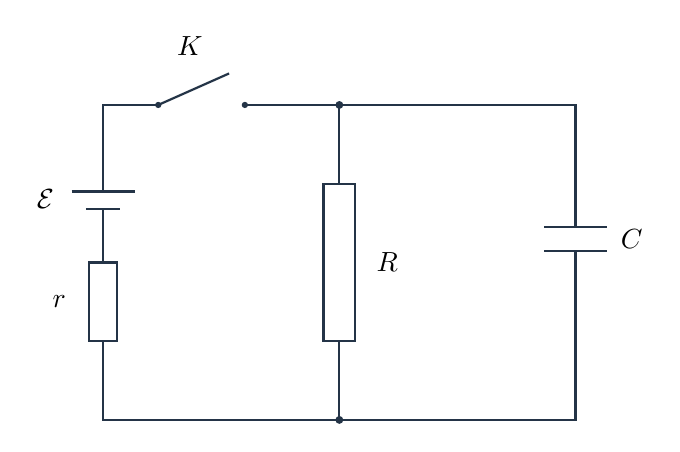
\begin{tikzpicture}
\draw[body](0,2.9)--(0,4)--(.7,4);\draw[body](1.8,4)--(6,4)--(6,2.45);
\draw[body](.7,4)--(1.6,4.4);\fill[ink](.7,4)circle(.04);\fill[ink](1.8,4)circle(.04);
\node[above]at(1.1,4.5){$K$};
\draw[body](-.4,2.9)--(.4,2.9);\draw[body](-.22,2.68)--(.22,2.68);
\draw[body](0,2.68)--(0,2);\draw[body](-.18,1)rectangle(.18,2);
\draw[body](0,1)--(0,0)--(6,0)--(6,2.15);
\draw[body](3,4)--(3,3);\draw[body](2.8,1)rectangle(3.2,3);\draw[body](3,1)--(3,0);
\draw[body](5.6,2.45)--(6.4,2.45);\draw[body](5.6,2.15)--(6.4,2.15);
\node[left]at(-.5,2.8){$\mathcal E$};\node[left]at(-.35,1.5){$r$};
\node[right]at(3.35,2){$R$};\node[right]at(6.45,2.3){$C$};
\fill[ink](3,4)circle(.05);\fill[ink](3,0)circle(.05);
\end{tikzpicture}
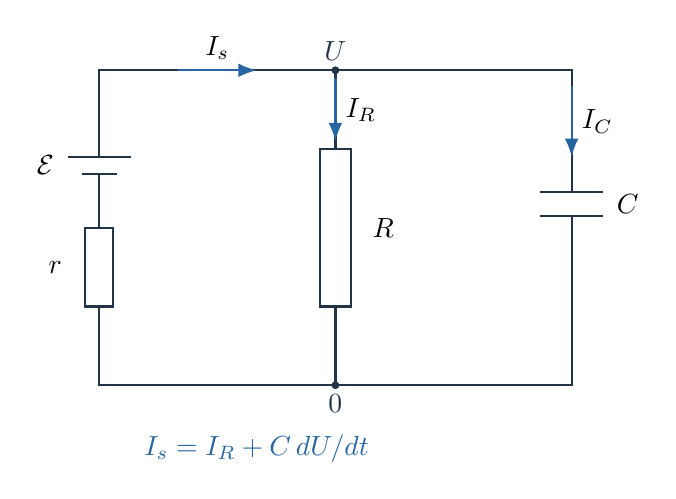
\begin{tikzpicture}
\draw[body](0,2.9)--(0,4)--(6,4)--(6,2.45);
\draw[body](-.4,2.9)--(.4,2.9);\draw[body](-.22,2.68)--(.22,2.68);
\draw[body](0,2.68)--(0,2);\draw[body](-.18,1)rectangle(.18,2);
\draw[body](0,1)--(0,0)--(6,0)--(6,2.15);
\draw[body](3,4)--(3,3);\draw[body](2.8,1)rectangle(3.2,3);\draw[body](3,1)--(3,0);
\draw[body](5.6,2.45)--(6.4,2.45);\draw[body](5.6,2.15)--(6.4,2.15);
\node[left]at(-.45,2.8){$\mathcal E$};\node[left]at(-.35,1.5){$r$};
\node[right]at(3.35,2){$R$};\node[right]at(6.45,2.3){$C$};
\draw[vec](1,4)--(2,4)node[midway,above]{$I_s$};
\draw[vec](3,3.9)--(3,3.1)node[midway,right]{$I_R$};
\draw[vec](6,3.8)--(6,2.9)node[midway,right]{$I_C$};
\fill[ink](3,4)circle(.05)node[above]{$U$};\fill[ink](3,0)circle(.05)node[below]{$0$};
\node[blue]at(2,-.8){$I_s=I_R+C\,dU/dt$};
\end{tikzpicture}
\begin{tikzpicture}
\node at(1.5,4.2){闭合等效};\node at(6.8,4.2){断开放电};
\draw[body](0,2.2)--(0,3)--(1,3);
\draw[body](1,2.8)rectangle(2.2,3.2);\draw[body](2.2,3)--(3.2,3)--(3.2,1.6);
\draw[body](-.35,2.2)--(.35,2.2);\draw[body](-.2,2)--(.2,2);
\draw[body](0,2)--(0,.5)--(3.2,.5)--(3.2,1.3);
\draw[body](2.85,1.6)--(3.55,1.6);\draw[body](2.85,1.3)--(3.55,1.3);
\node[left]at(-.4,2.1){$U_e$};\node[above]at(1.6,3.2){$r\parallel R$};
\node[right]at(3.6,1.45){$C$};\node at(1.6,-.25){$\tau_c=(r\parallel R)C$};
\draw[body](5.5,2.5)--(5.5,3)--(8.3,3)--(8.3,1.6);
\draw[body](5.3,1.2)rectangle(5.7,2.5);\draw[body](5.5,1.2)--(5.5,.5)--(8.3,.5)--(8.3,1.3);
\draw[body](7.95,1.6)--(8.65,1.6);\draw[body](7.95,1.3)--(8.65,1.3);
\node[left]at(5.1,1.8){$R$};\node[right]at(8.7,1.45){$C$};
\node at(6.9,-.25){$\tau_d=RC$};
\end{tikzpicture}
\begin{tikzpicture}
\node[draw=ink,rounded corners,minimum width=2cm,minimum height=1cm](S)at(0,1){电源 $W$};
\node[draw=ink,rounded corners,minimum width=2.5cm,minimum height=1cm](H)at(5,2){闭合段热量};
\node[draw=ink,rounded corners,minimum width=2.5cm,minimum height=1cm](C)at(5,0){电容储能增加};
\node[draw=ink,rounded corners,minimum width=2.5cm,minimum height=1cm](D)at(9,0){断开段热量};
\draw[vec](S.east)--(H.west);\draw[vec](S.east)--(C.west);
\draw[vec](C.east)--(D.west);
\node at(5,-1.5){稳态一周期：$\Delta E_C=0$，电源功等于两阶段总热};
\end{tikzpicture}
\end{document}
